\documentclass[12pt]{article}
\usepackage[utf8]{inputenc}
\usepackage{geometry}
\geometry{legalpaper, margin=1in, top=10mm}
\usepackage{graphicx}
\usepackage{caption}
\usepackage[export]{adjustbox}
\usepackage{mathptmx}
\usepackage{secdot}
\usepackage{amsmath}

%\usepackage{subfig}
\usepackage[framed,numbered,autolinebreaks,useliterate]{mcode}
\usepackage{xcolor}
\usepackage{listings}
\usepackage{subcaption}
\usepackage{mwe}

\definecolor{mGreen}{rgb}{0,0.6,0}
\definecolor{mGray}{rgb}{0.5,0.5,0.5}
\definecolor{mPurple}{rgb}{0.58,0,0.82}
\definecolor{backgroundColour}{rgb}{0.95,0.95,0.92}

\usepackage{hyperref}
\newcommand\Tstrut{\rule{0pt}{2.6ex}}         % = `top' strut
\newcommand\Bstrut{\rule[-0.9ex]{0pt}{0pt}}   % = `bottom' strut
\AtBeginDocument{\hypersetup{pdfborder={0 0 1}}}
\lstdefinestyle{CStyle}{
	backgroundcolor=\color{white},   
	commentstyle=\color{mGreen},
	keywordstyle=\color{magenta},
	numberstyle=\tiny\color{mGray},
	stringstyle=\color{mPurple},
	basicstyle=\footnotesize,
	breakatwhitespace=false,         
	breaklines=true,                 
	captionpos=b,                    
	keepspaces=true,                 
	numbers=left,                    
	numbersep=5pt,                  
	showspaces=false,                
	showstringspaces=false,
	showtabs=false,                  
	tabsize=2,
	language=C
}
\title{%
	Edge Dectection, Template Matching and Blob Coloring \\
	\large Homework 3 }

\author{Jinaykumar Patel \\ 1001937580}

\date{}
\begin{document}
	\maketitle
	
\section{Implement Edge Detection Using Prewit Templates}

$$
\operatorname{vert.:}\left[\begin{array}{lll}
	-1 & 0 & 1 \\
	-1 & 0 & 1 \\
	-1 & 0 & 1
\end{array}\right] \hspace{1.2cm}\text {min. diag.: }\left[\begin{array}{ccc}
-1 & -1 & 0 \\
-1 & 0 & 1 \\
0 & 1 & 1
\end{array}\right]
$$
$$
\operatorname{hor.: }\left[\begin{array}{ccc}
	-1 & -1 & -1 \\
	0 & 0 & 0 \\
	1 & 1 & 1
\end{array}\right] \hspace{0.8cm} \text {maj. diag.:}\left[\begin{array}{ccc}
	0 & -1 & -1 \\
	1 & 0 & -1 \\
	1 & 1 & 0
\end{array}\right] 
$$
Edge detection is implemented using convolution with the four Prewit templates shown above. Each template is implemented separtely and results for each templates are saved in PNG files as\\
\textit{\textbf{p1\_chess\_}\{template\_name\}} and \textit{\textbf{p1\_nedderman\_}\{template\_name\}}.
The results obtained from edge detection implementation in Chess and Nedderman images are shown in Fig. \ref{fig:edge_detect} and Fig. \ref{fig:edge_detect2}, respectively.


\begin{figure*}
	\centering
	\begin{subfigure}[b]{0.475\textwidth}
		\centering
		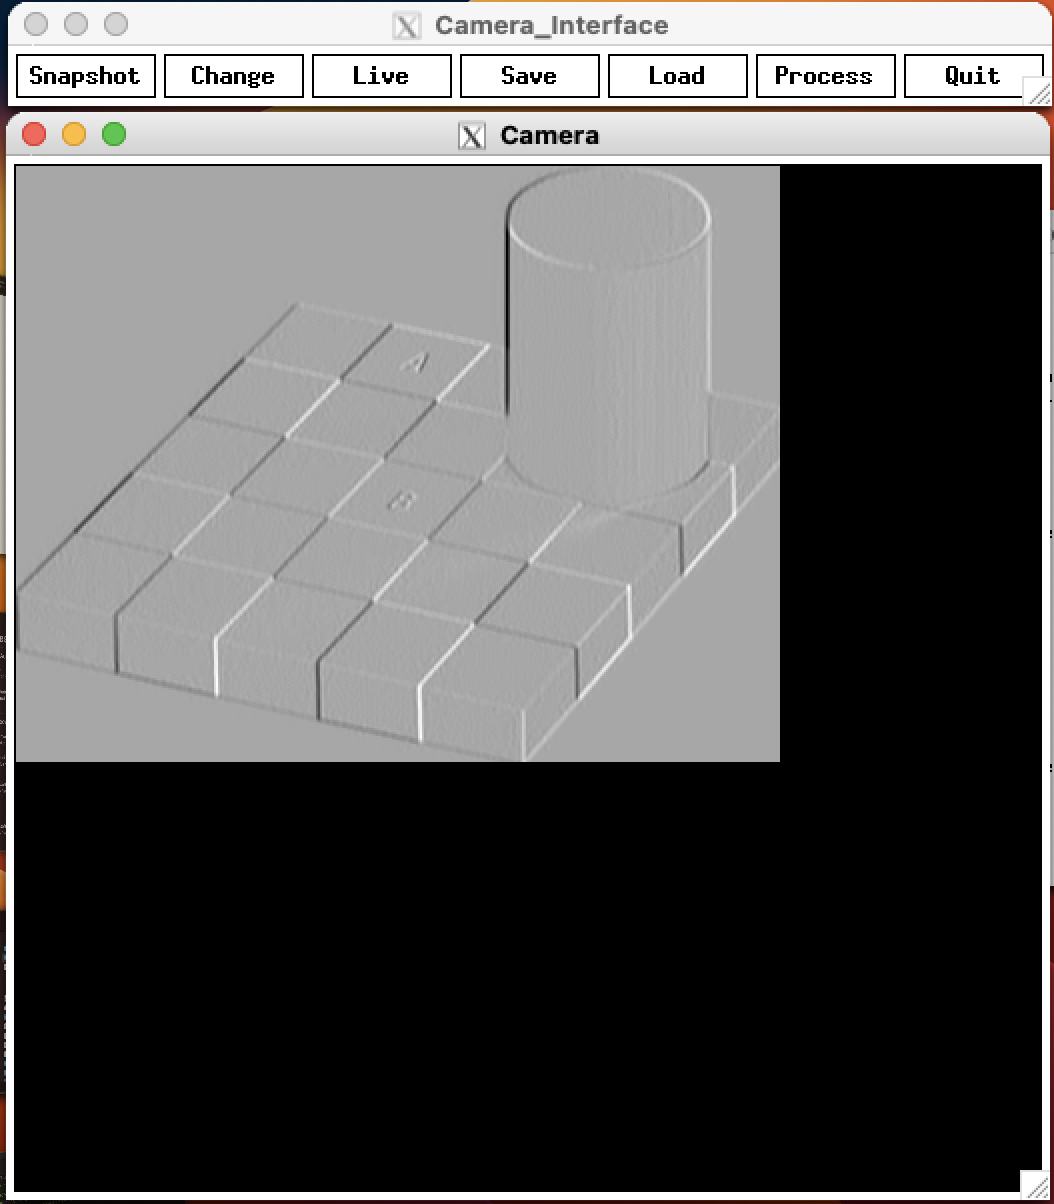
\includegraphics[width=\textwidth]{hw3_results/p1_chess_hor}
		\caption[]%
		{{\small Horizontal Template}}    
		\label{fig:mean and std of net14}
	\end{subfigure}
	\hfill
	\begin{subfigure}[b]{0.475\textwidth}  
		\centering 
		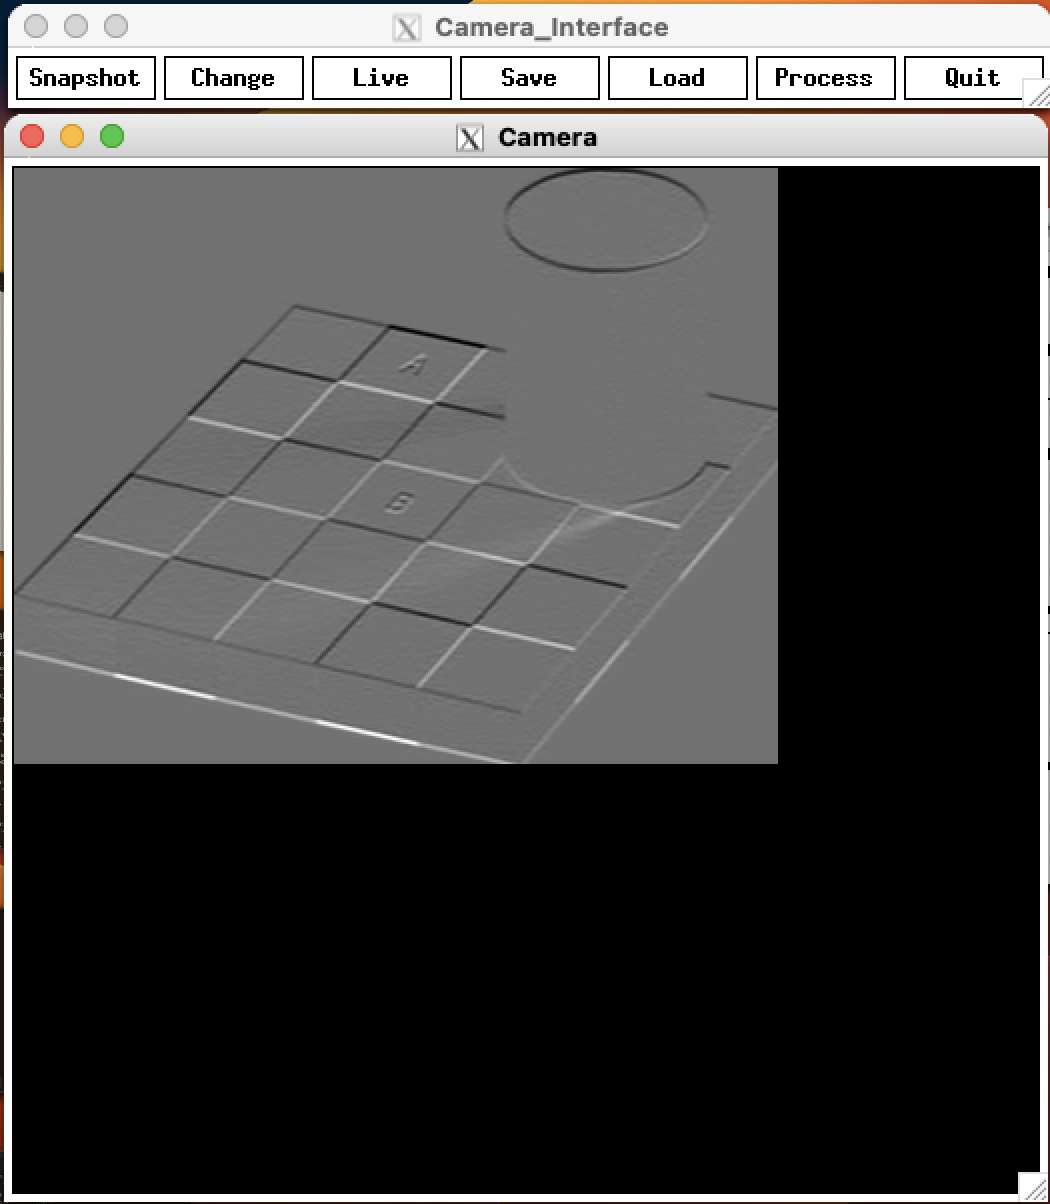
\includegraphics[width=\textwidth]{hw3_results/p1_chess_vert}
		\caption[]%
		{{\small Vertical Template}}    
		\label{fig:mean and std of net24}
	\end{subfigure}
	\vskip\baselineskip
	\begin{subfigure}[b]{0.475\textwidth}   
		\centering 
		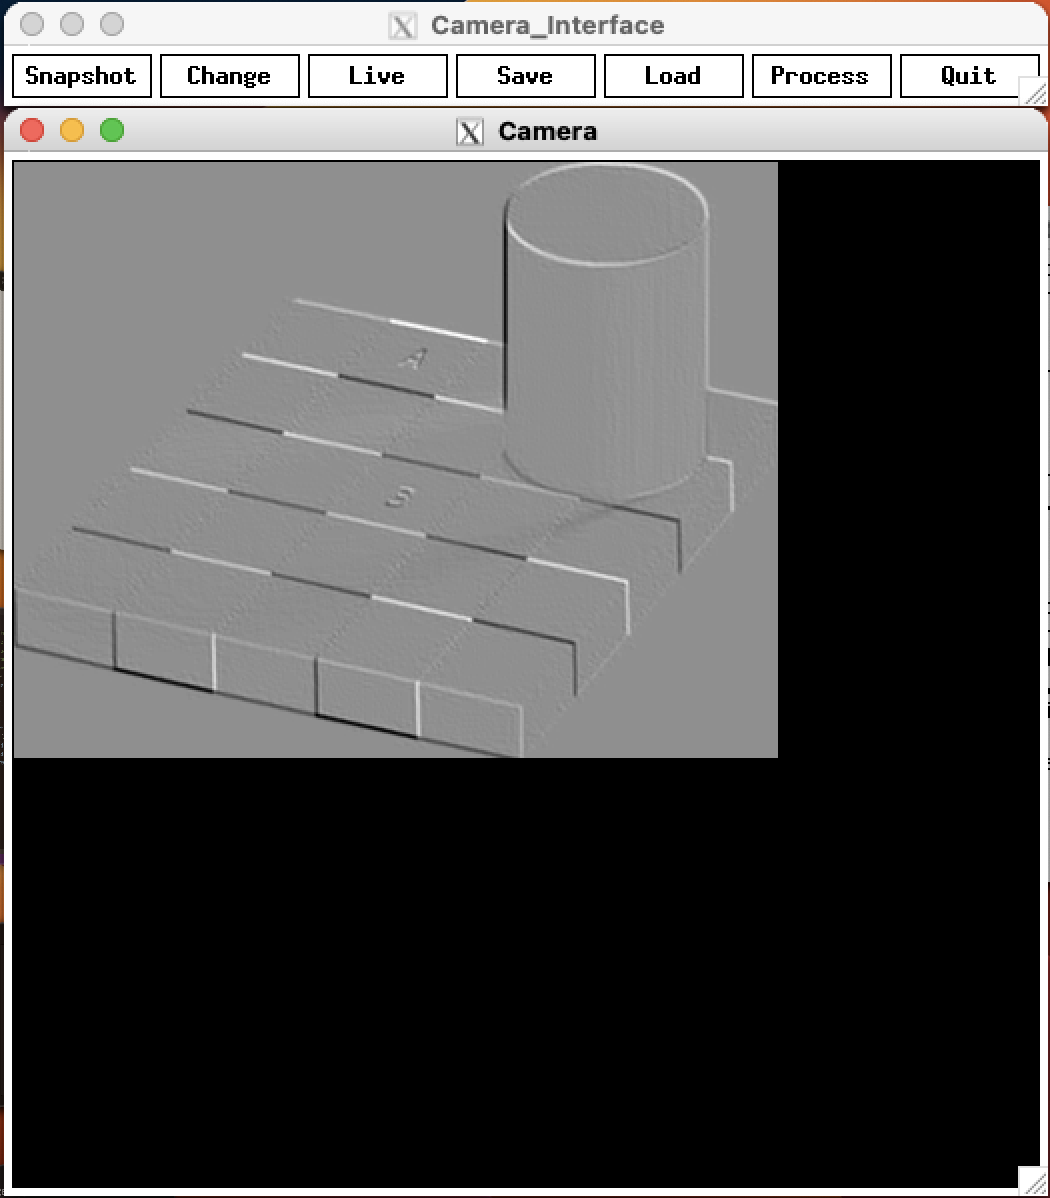
\includegraphics[width=\textwidth]{hw3_results/p1_chess_majdiag}
		\caption[]%
		{{\small Maj. diag Template}}    
		\label{fig:mean and std of net34}
	\end{subfigure}
	\hfill
	\begin{subfigure}[b]{0.475\textwidth}   
		\centering 
		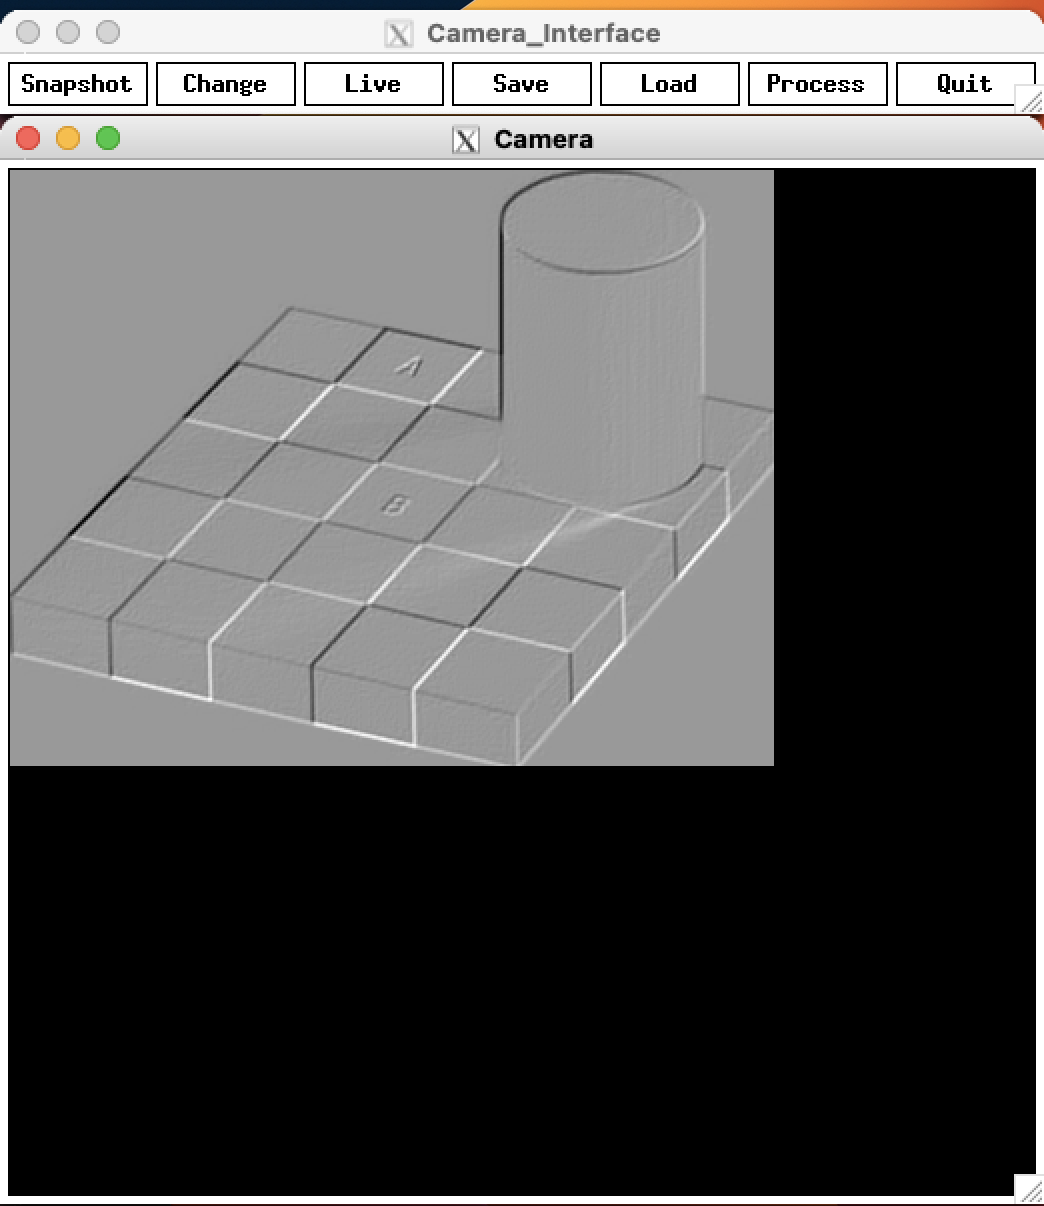
\includegraphics[width=\textwidth]{hw3_results/p1_chess_mindiag}
		\caption[]%
		{{\small Min. diag Template}}    
		\label{fig:mean and std of net44}
	\end{subfigure}
	\caption[ ]
	{\small Edge Detection (Chess) using Prewit Templates} 
	\label{fig:edge_detect}
\end{figure*}

\begin{figure*}
	\centering
	\begin{subfigure}[b]{0.475\textwidth}
		\centering
		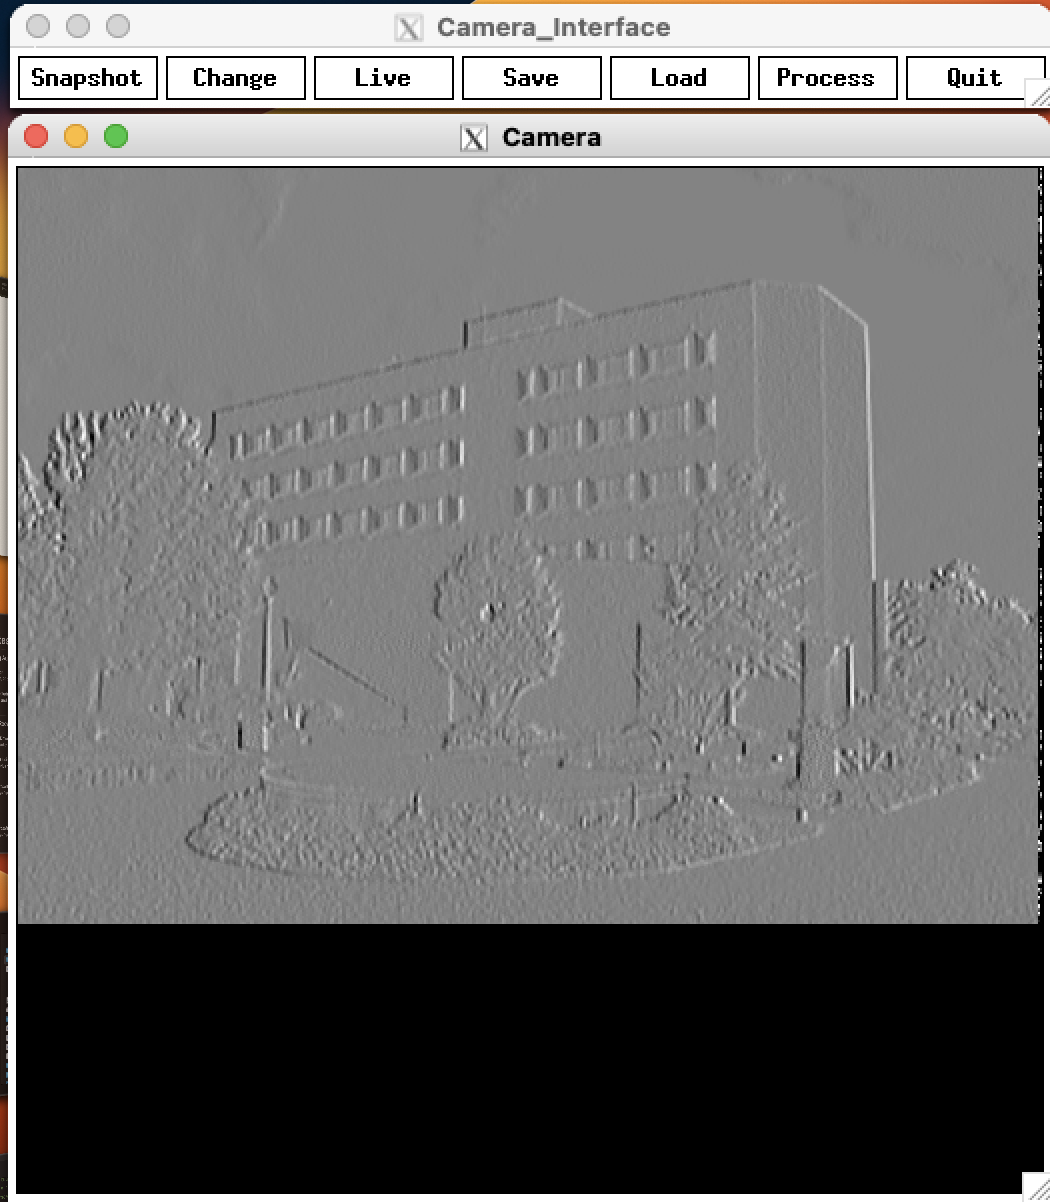
\includegraphics[width=\textwidth]{hw3_results/p1_nedd_hor}
		\caption[]%
		{{\small Horizontal Template}}    
		\label{fig:mean and std of net12}
	\end{subfigure}
	\hfill
	\begin{subfigure}[b]{0.475\textwidth}  
		\centering 
		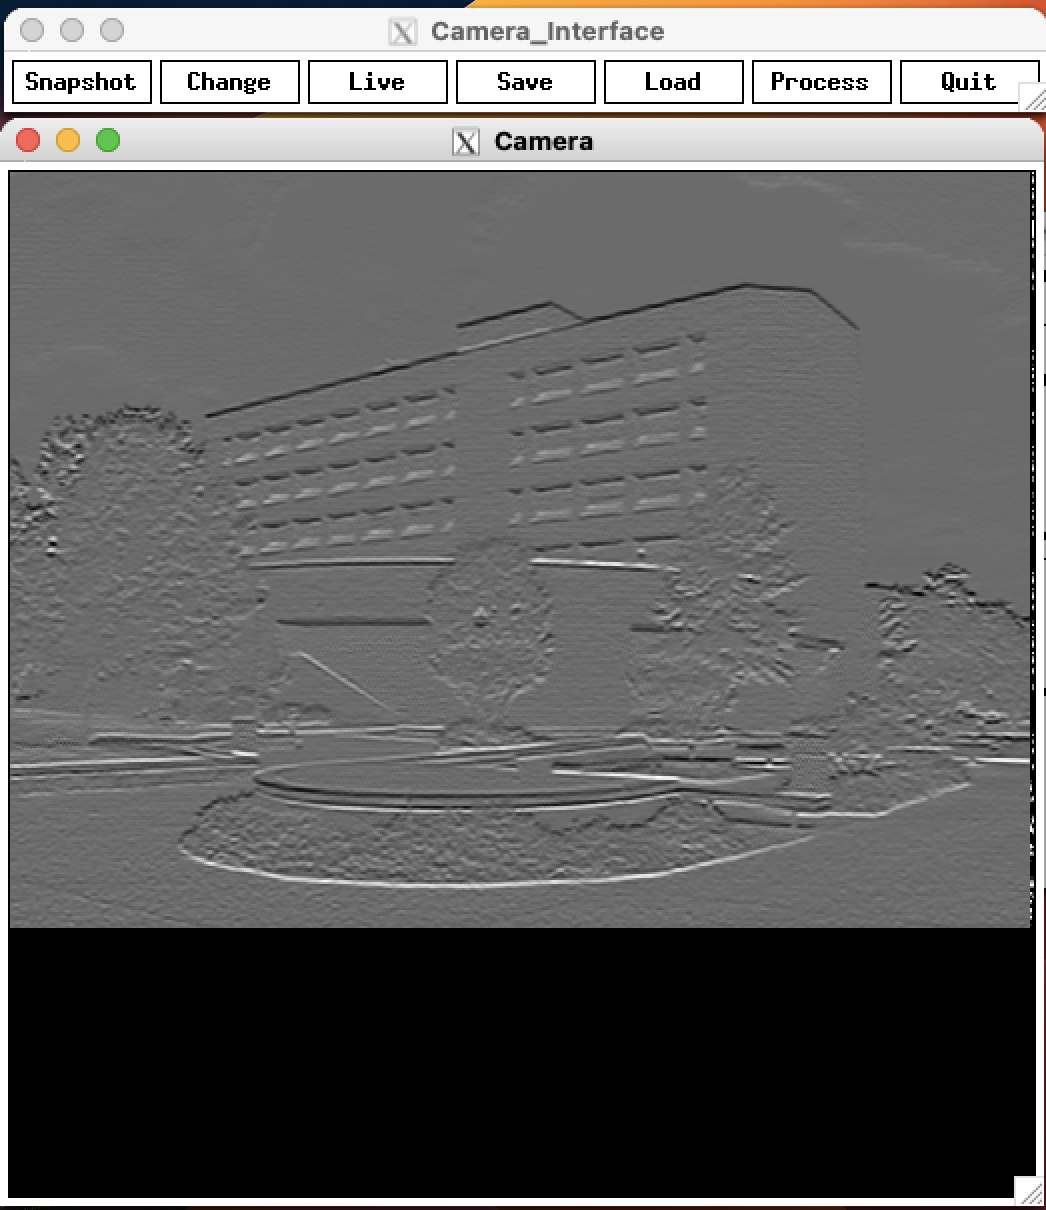
\includegraphics[width=\textwidth]{hw3_results/p1_nedd_vert}
		\caption[]%
		{{\small Vertical Template}}    
		\label{fig:mean and std of net22}
	\end{subfigure}
	\vskip\baselineskip
	\begin{subfigure}[b]{0.475\textwidth}   
		\centering 
		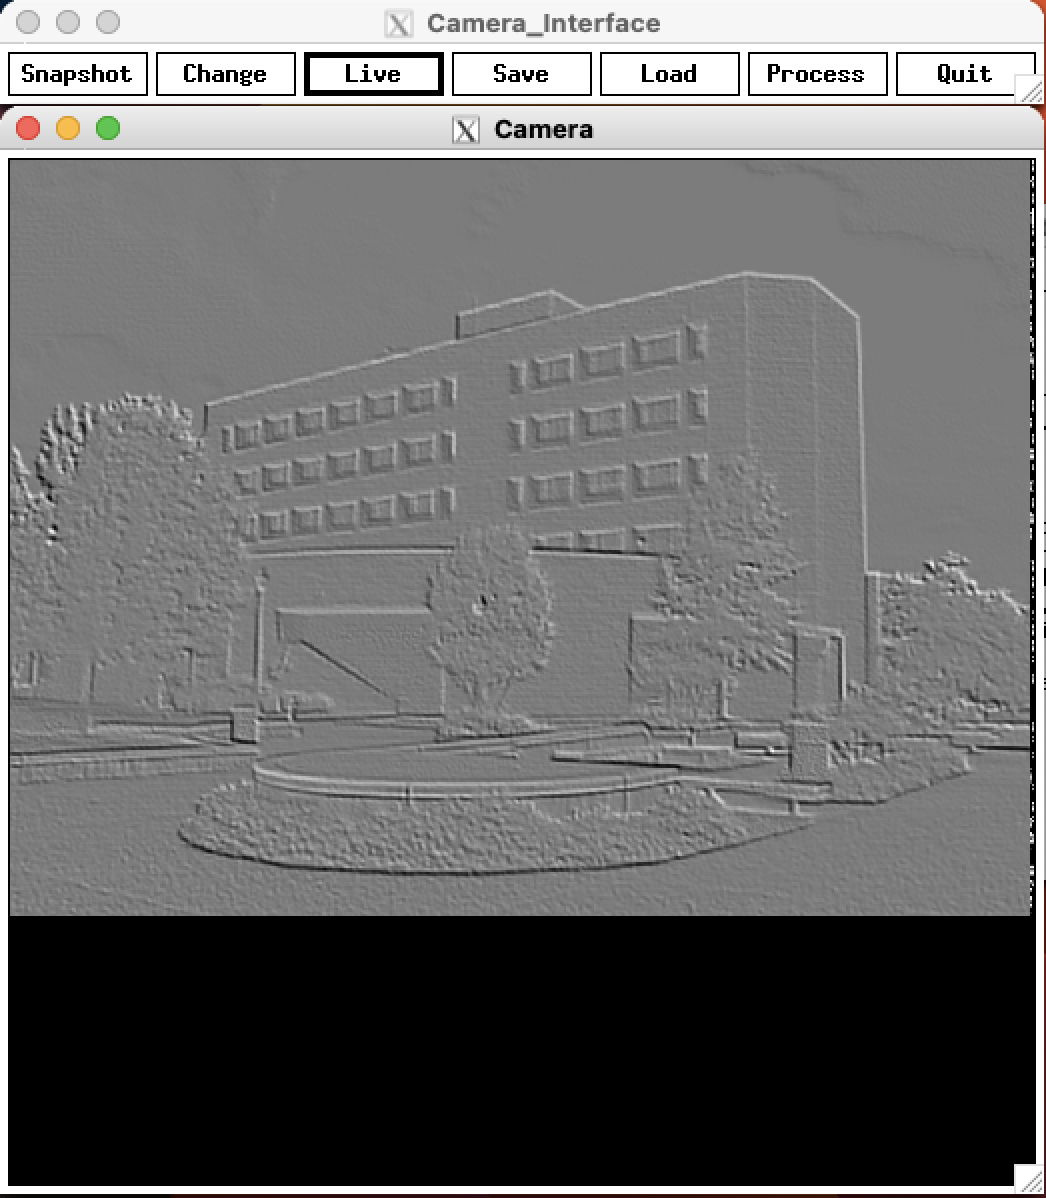
\includegraphics[width=\textwidth]{hw3_results/p1_nedd_majdiag}
		\caption[]%
		{{\small Maj. diag Template}}    
		\label{fig:mean and std of net32}
	\end{subfigure}
	\hfill
	\begin{subfigure}[b]{0.475\textwidth}   
		\centering 
		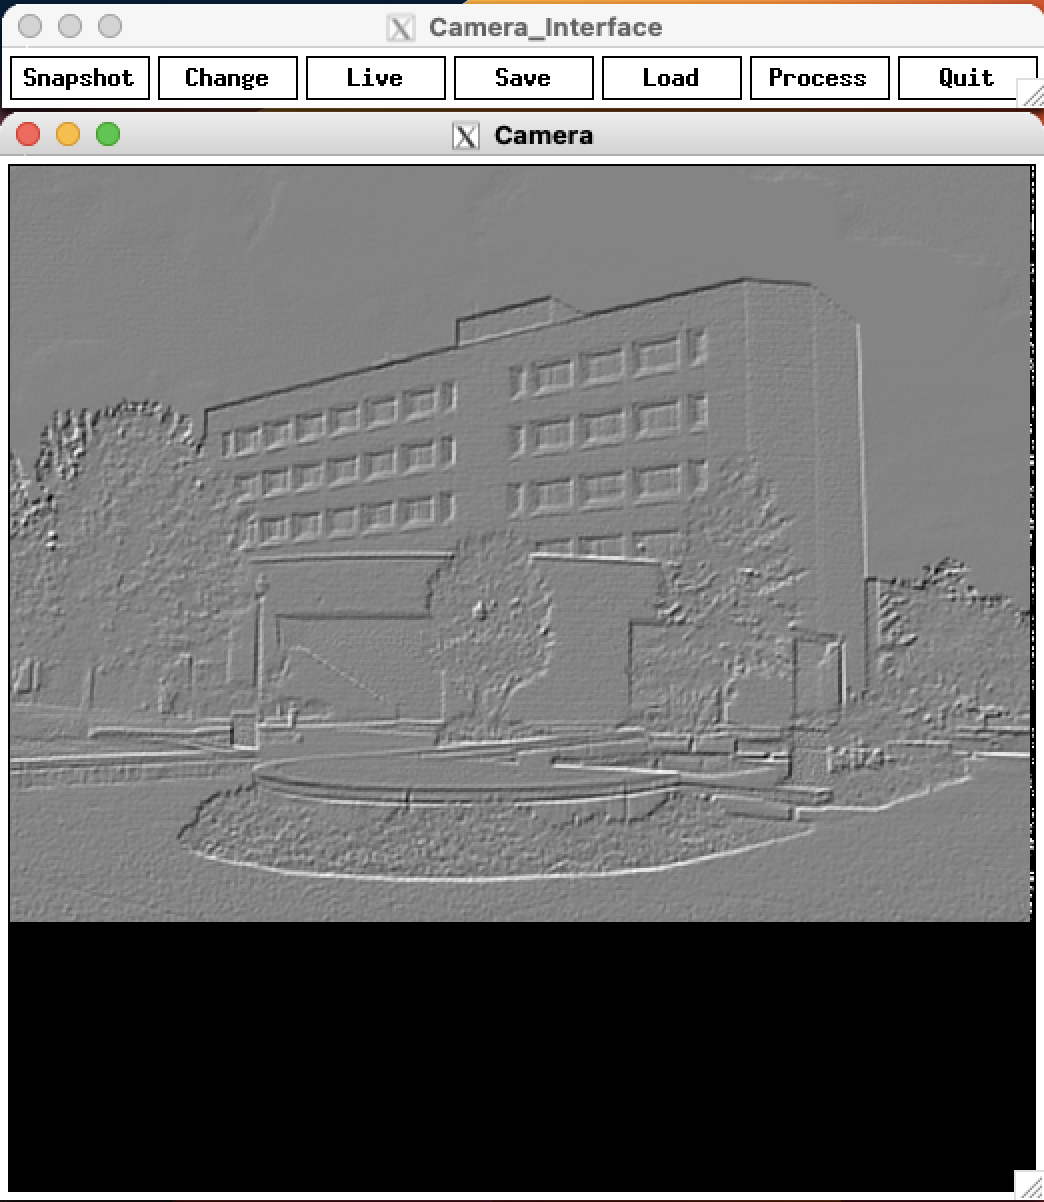
\includegraphics[width=\textwidth]{hw3_results/p1_nedd_mindiag}
		\caption[]%
		{{\small Min. diag Template}}    
		\label{fig:mean and std of net42}
	\end{subfigure}
	\caption[ ]
	{\small Edge Detection (Nedderman) using Prewit Templates} 
	\label{fig:edge_detect2}
\end{figure*}


\section{Implement Template Matching Using Normalized Convolution}
Here a specific region is chosen and is used as the template i.e. finding all instances of similar objects in the image. Template matching is implemented using this template with the use of normalized cross correlation (convolution
which adjusts for the image and template means as well as for the image and template variances - i.e. contrast). The result of the convolution is written back into the result image, normalizing the values to be between 0 and 255. 

Two templates are chosen in the nedderman images:
\begin{itemize}
	\item[1.] \underline{ \textbf{Small windows}} in the nedderman buildings are selected as template and used for template matching. The results is shown in Fig. \ref{fig:ned_temp}. We can see the bright regions in the Fig. \ref{fig:ned_result} where the windows are in the original image.
	\item[2.] \underline{\textbf{Tree}} in the middle of the image is selected as a template. The result is shown in Fig. \ref{fig:ned_temp2}. We can see the bright spot in the place of the tree in the middle (Fig. \ref{fig:ned_result2}).

\end{itemize}
Now, chess image is used. A corner between white and black spots is chosen as the template and template matching is implemented. The results are shown in Fig. \ref{fig:chess_temp}. We can see that some white corners and some black corners in Fig. \ref{fig:chess_result}. Black corner are the ones which are exactly opposite to the region selected as the template.  
\begin{figure*}
	\centering
	\begin{subfigure}[b]{0.475\textwidth}
		\centering
		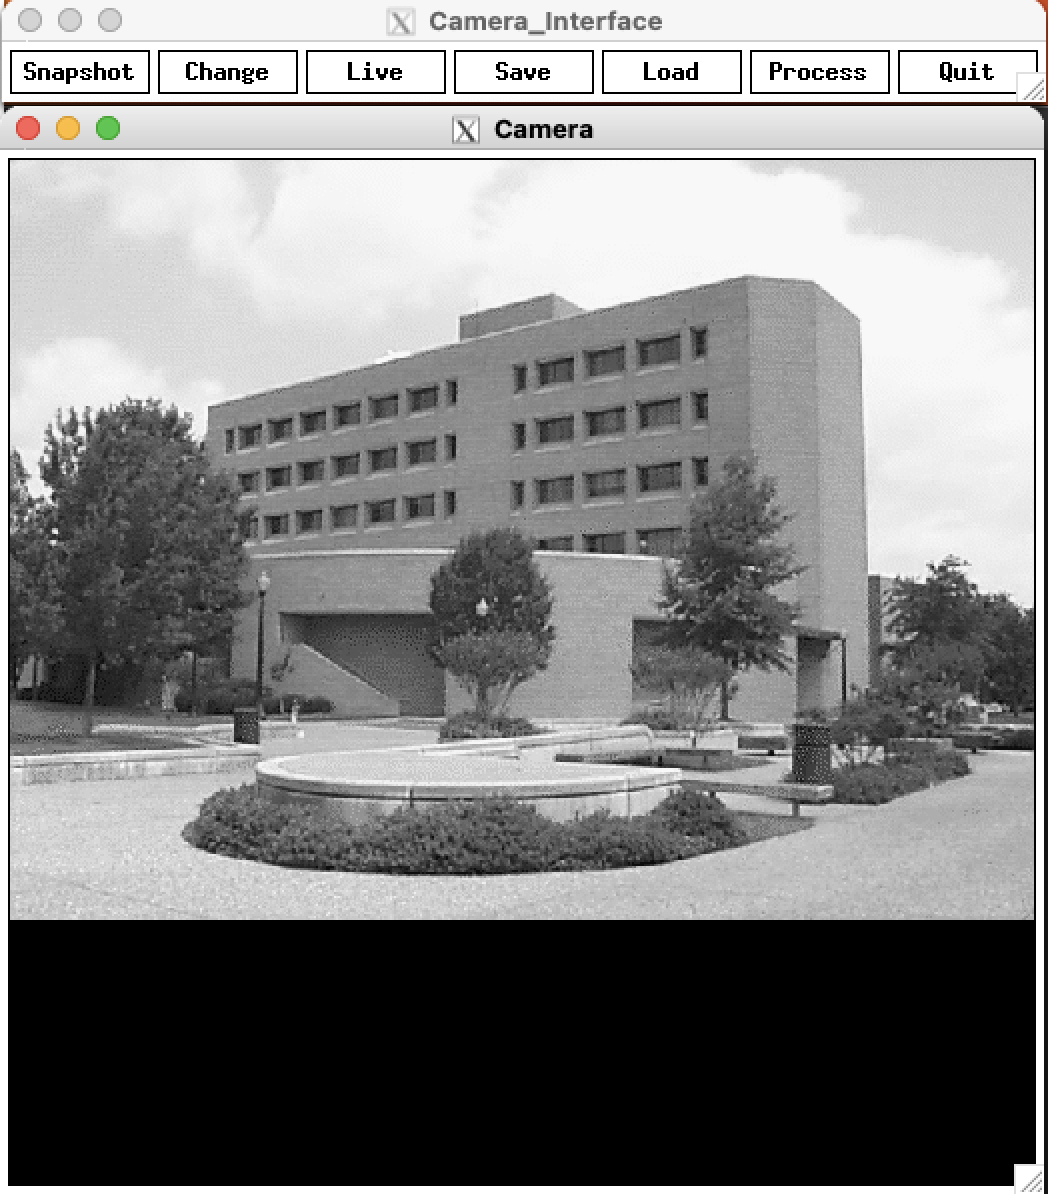
\includegraphics[width=\textwidth]{hw3_results/nedderman}
		\caption[]%
		{{\small Nedderman Image}}    
		\label{fig:ned}
	\end{subfigure}
	\hfill
	\begin{subfigure}[b]{0.475\textwidth}  
		\centering 
		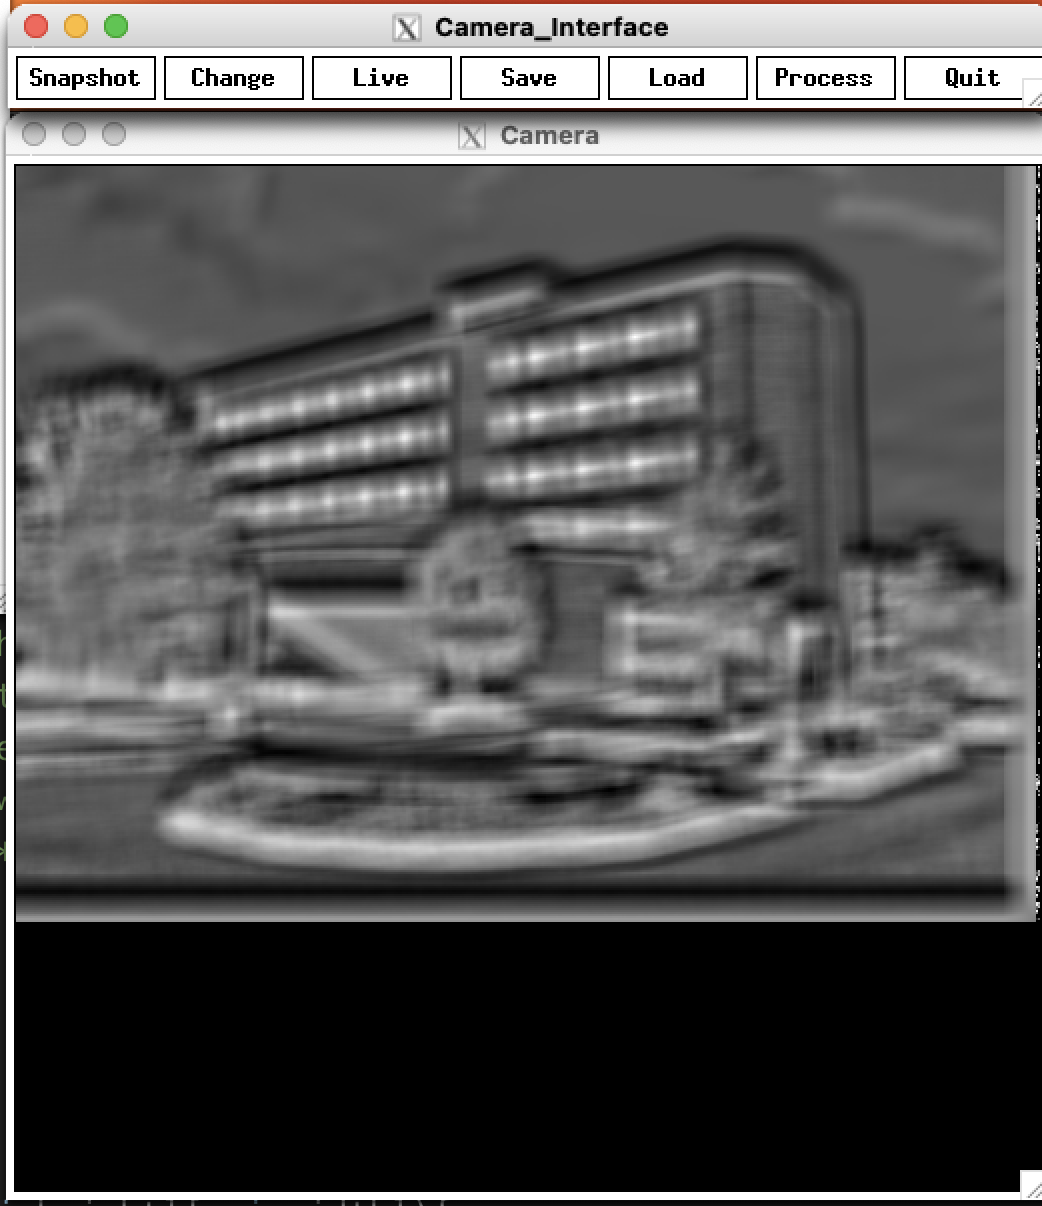
\includegraphics[width=\textwidth]{hw3_results/p2_window_template}
		\caption[]%
		{{\small Image after template matching}}    
		\label{fig:ned_result}
	\end{subfigure}
	\caption[ ]
	{\small Template Matching (Window as a template)} 
	\label{fig:ned_temp}
\end{figure*}

\begin{figure*}
	\centering
	\begin{subfigure}[b]{0.475\textwidth}
		\centering
		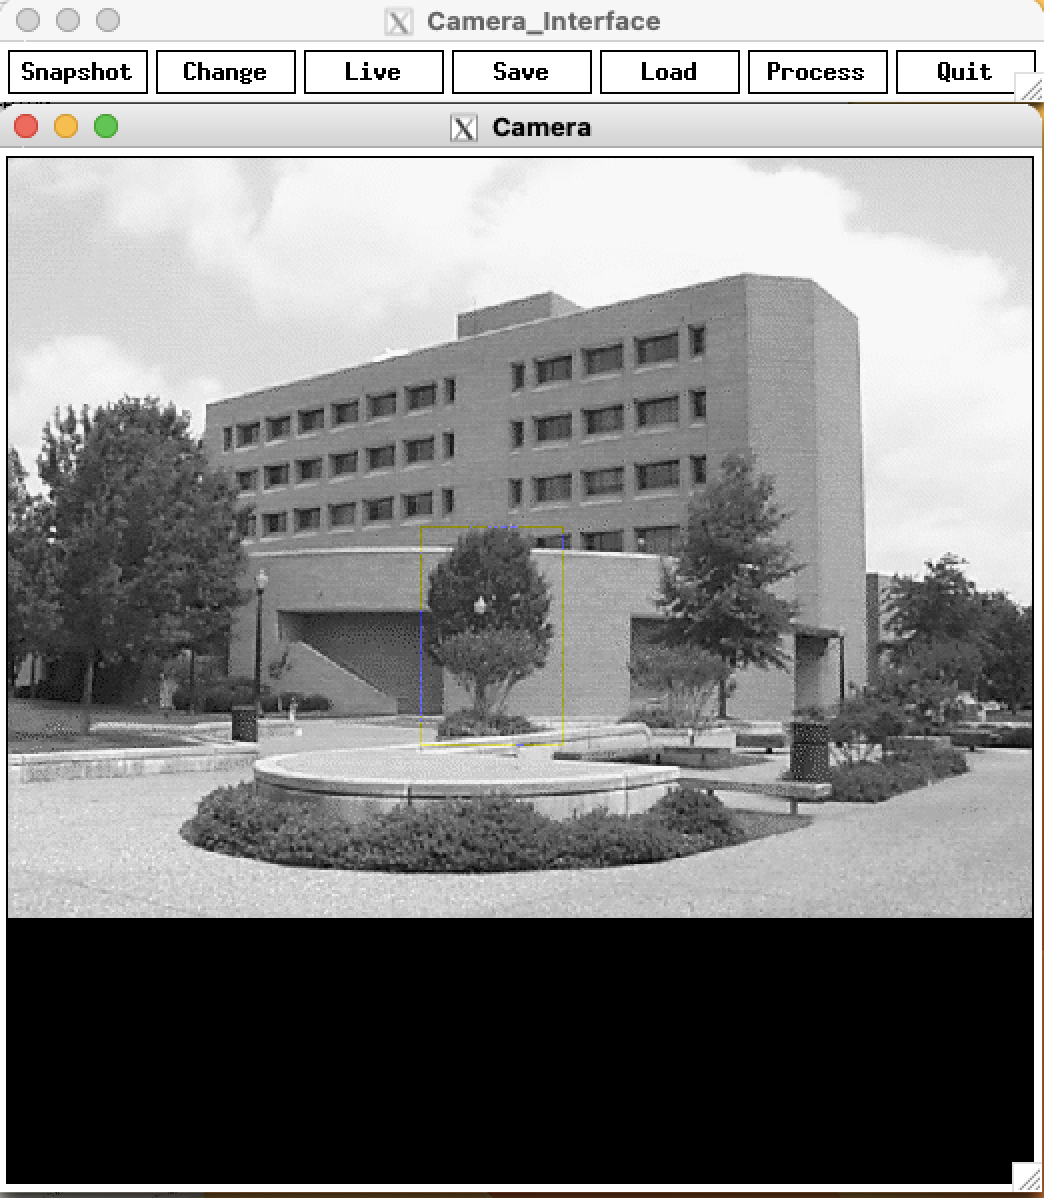
\includegraphics[width=\textwidth]{hw3_results/nedderman_tree_select}
		\caption[]%
		{{\small Nedderman Image}}    
		\label{fig:ned2}
	\end{subfigure}
	\hfill
	\begin{subfigure}[b]{0.475\textwidth}  
		\centering 
		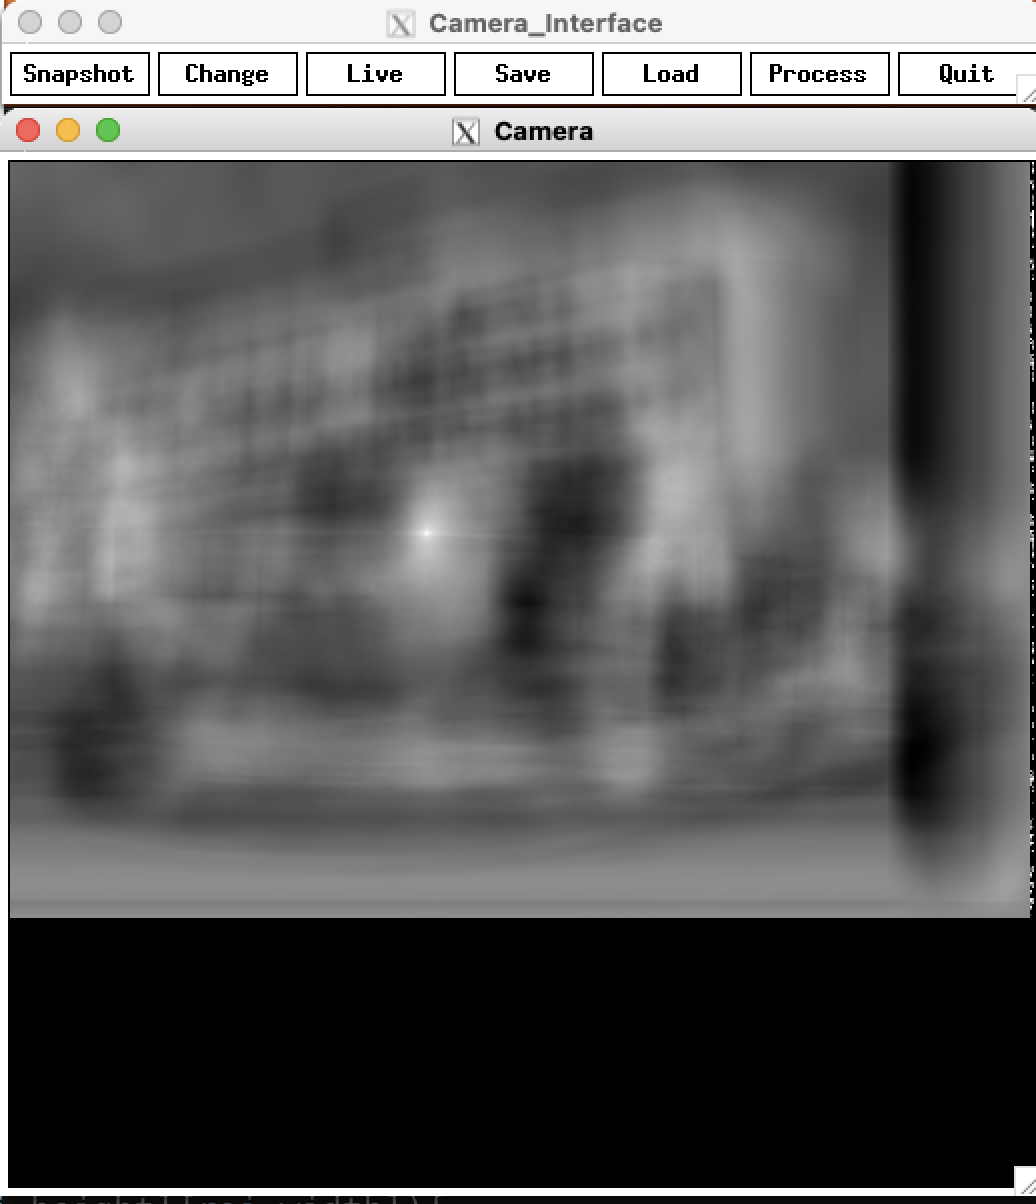
\includegraphics[width=\textwidth]{hw3_results/p2_tree_template}
		\caption[]%
		{{\small Image after template matching}}    
		\label{fig:ned_result2}
	\end{subfigure}
	\caption[ ]
	{\small Template Matching (Tree as a template)} 
	\label{fig:ned_temp2}
\end{figure*}

\begin{figure*}
	\centering
	\begin{subfigure}[b]{0.475\textwidth}
		\centering
		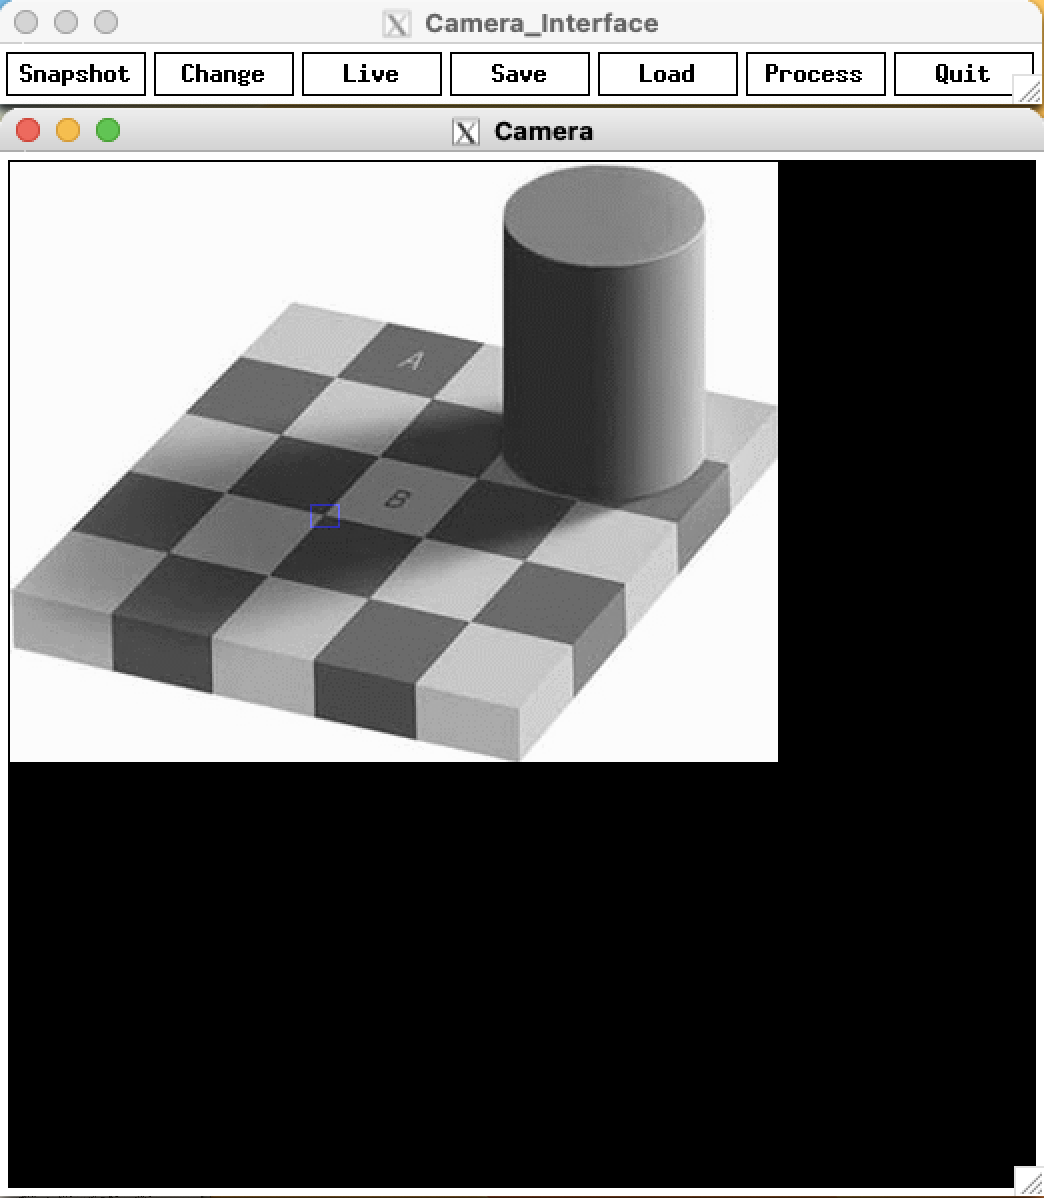
\includegraphics[width=\textwidth]{hw3_results/chess_corner_temp}
		\caption[]%
		{{\small Chess Image}}    
		\label{fig:chess}
	\end{subfigure}
	\hfill
	\begin{subfigure}[b]{0.475\textwidth}  
		\centering 
		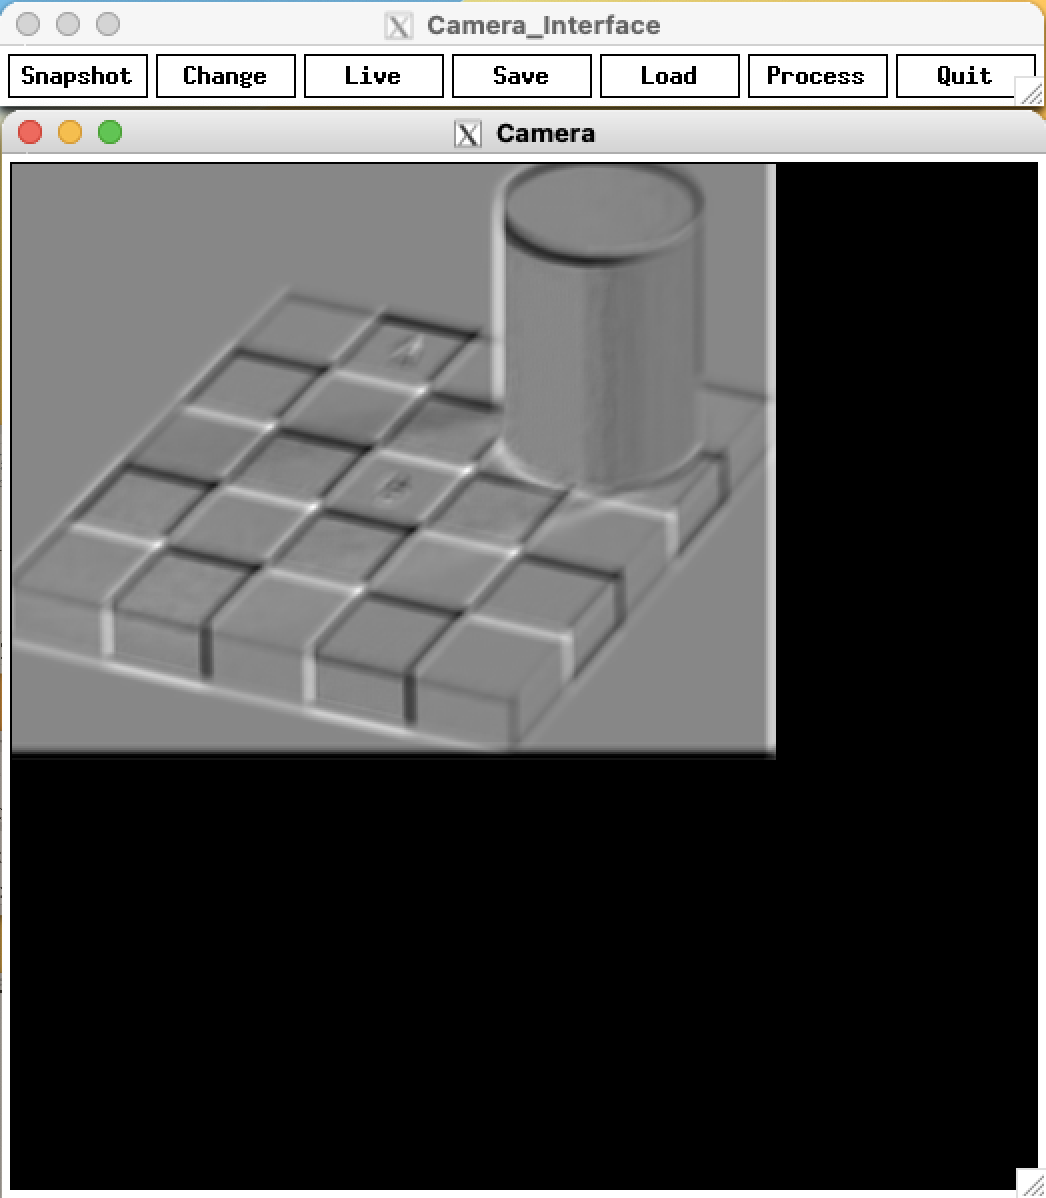
\includegraphics[width=\textwidth]{hw3_results/p2_chess_corner_template}
		\caption[]%
		{{\small Image after template matching}}    
		\label{fig:chess_result}
	\end{subfigure}
	\caption[ ]
	{\small Template Matching (Corner as a template)} 
	\label{fig:chess_temp}
\end{figure*}

\section{Implement Segmentation Using Blob Coloring}
Blob coloring is implemented to identify regions with a common intensity in the
image. Here the threshold between the pixels is chosen to be 10. This value can be changed in the threshold function. Fig. \ref{fig:blocks_temp} shows the result obtain when blob coloring algorithm is implemented. There are some small dotted regions appearing in the resulted image which I am not aware of. 
\begin{figure*}
	\centering
	\begin{subfigure}[b]{0.475\textwidth}
		\centering
		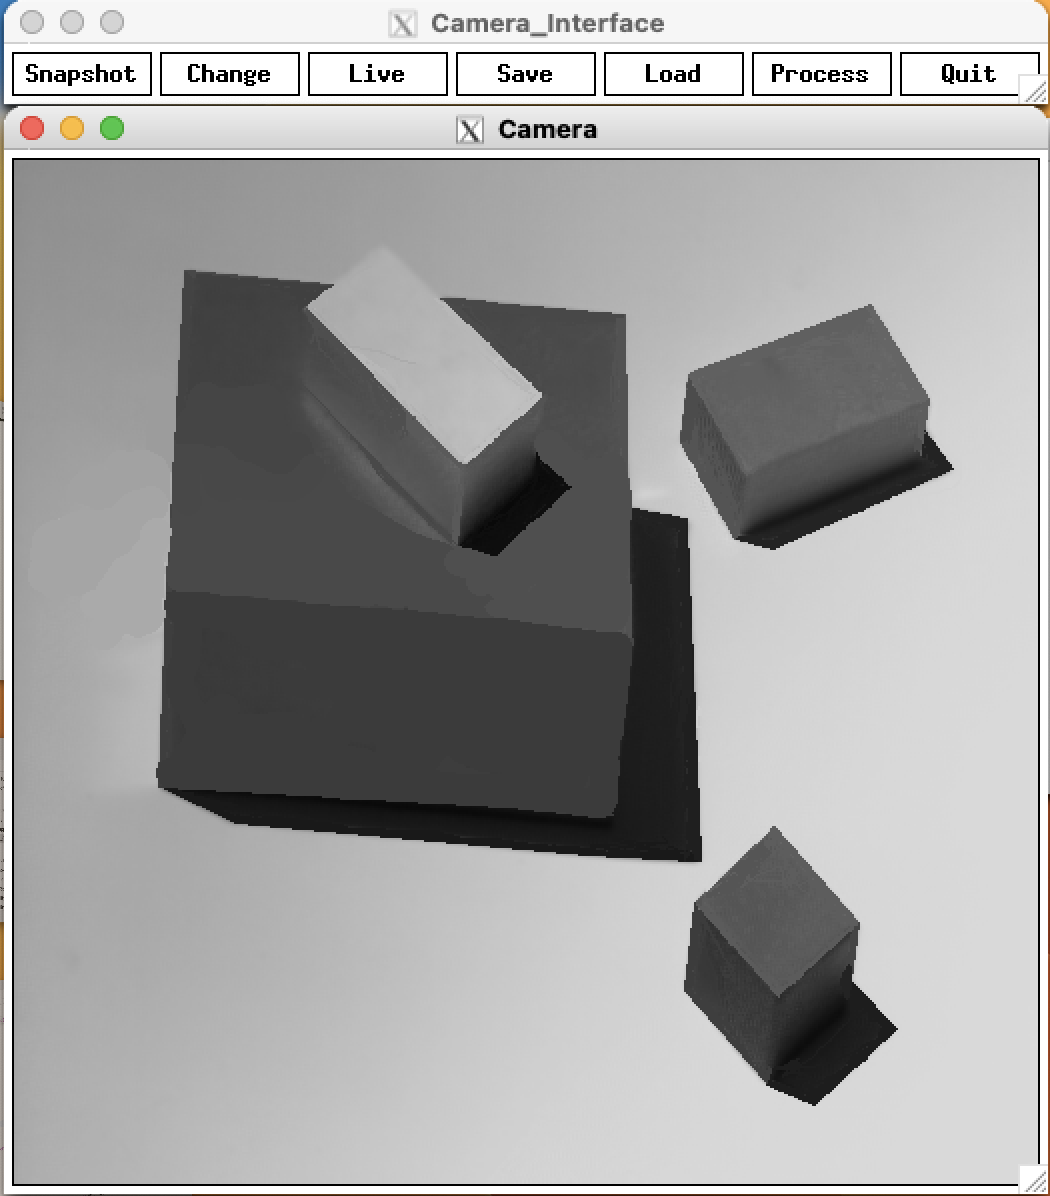
\includegraphics[width=\textwidth]{hw3_results/blocks}
		\caption[]%
		{{\small Blocks Image}}    
		\label{fig:blocks}
	\end{subfigure}
	\hfill
	\begin{subfigure}[b]{0.475\textwidth}  
		\centering 
		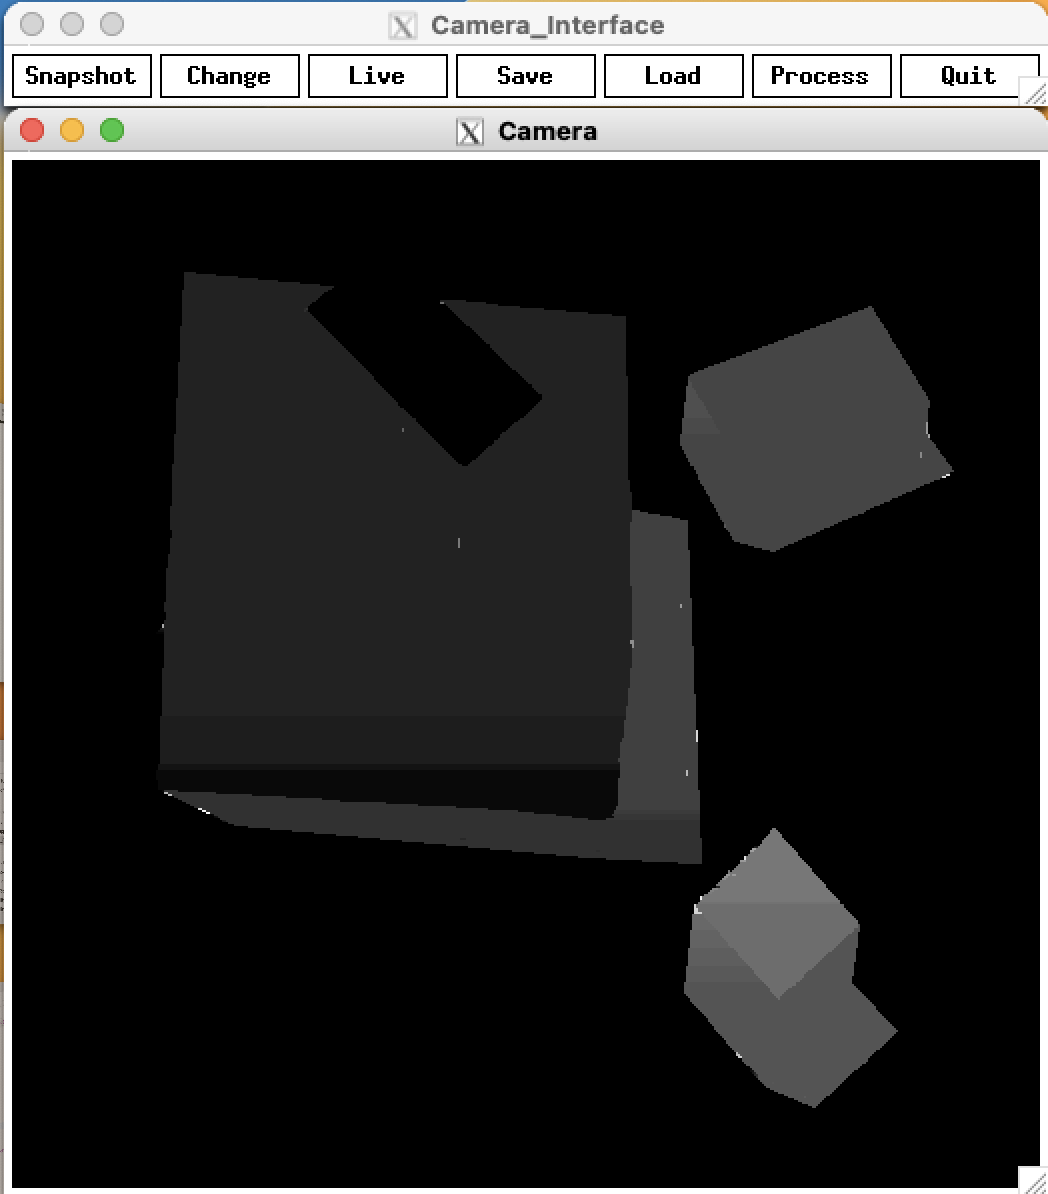
\includegraphics[width=\textwidth]{hw3_results/p3_blocks}
		\caption[]%
		{{\small Image after blob coloring}}    
		\label{fig:blocks_result}
	\end{subfigure}
	\caption[ ]
	{\small Blob coloring} 
	\label{fig:blocks_temp}
\end{figure*}

\end{document}

